\chapter{Objetivos}
\label{cap:capitulo3}

\begin{flushright}
\begin{minipage}[]{10cm}
\emph{El éxito es la suma de pequeños esfuerzos repetidos día tras día.}\\
\end{minipage}\\

Robert Collier\\
\end{flushright}

\vspace{1cm}

Una vez establecido el marco contextual en los capítulos anteriores, en este capítulo se presentan los objetivos que se han marcado en este proyecto, así como los requisitos necesarios para su desarrollo.
Además, se describe la metodología empleada y el plan de trabajo que se ha llevado a cabo.\\

\section{Descripción del problema}
\label{sec:descripcion}
El incremento de la población envejecida con deterioro cognitivo ha generado una creciente necesidad de atención y cuidados especializados, recursos que no siempre están disponibles ni se adaptan a las necesidades de los usuarios. Esta falta de atención continua e individualizada tiene como consecuencia la dificultad para mantener sus capacidades cognitivas y una adecuada calidad de vida.

Esta situación no solo afecta a la calidad de vida de los usuarios, sino que también supone una carga para su entorno cercano y sus cuidadores, evidenciando así la necesidad de soluciones de apoyo.

\vspace{0.2cm}

En este contexto, el presente proyecto plantea el desarrollo de un robot de bajo coste orientado a ayudar a estas personas en su vida diaria, contribuyendo al mantenimiento de sus funciones cognitivas mediante juegos interactivos de estimulación. Asimismo, el robot proporciona una compañía activa a los usuarios, ayudando a mitigar la sensación de soledad y abandono mediante la interacción por voz basada en modelos de lenguaje.

La solución propuesta se plantea como un complemento a la atención personal tradicional, con el objetivo de reducir la carga de los cuidadores y fomentar la independencia del usuario. Con el fin de alcanzar este objetivo principal, se han establecido los siguientes subobjetivos:


\begin{enumerate}
	\item Investigar las soluciones existentes que cumplan con las características y objetivos establecidos.
	\item Explorar distintas estrategias para desarrollar juegos interactivos y la interfaz de usuario que no requieran un alto coste computacional.
	\item Estudiar y seleccionar componentes hardware y software de bajo coste disponibles en el mercado para el desarrollo del robot.
	\item Diseñar el modelo físico del robot usando herramientas de software libre como CAD (Computer-Aided Design).
	\item Hacer uso de impresora 3D para poder materializar las piezas del robot.
	\item Configurar la comunicación y conectividad del sistema para asegurar un funcionamiento correcto.
	\item Probar distintos algoritmos de reconocimiento facial.
	\item Investigar la eficacia de las LLMs (Large Language Models) según las necesidades.
	\item Integrar todos los componentes software en un sistema funcional.
    \item Realizar pruebas en un entorno real.
\end{enumerate}



\section{Requisitos}
\label{sec:Requisitos}

Una vez establecidos los subobjetivos, se deberán cumplir los siguientes requisitos:

\begin{enumerate}
	\item El sistema debe ejecutar algoritmos de bajo coste computacional para poder funcionar en una Raspberry Pi 4.
	\item Las librerías y software utilizados deben ser compatibles con Raspberry Pi 4.
	\item Los componentes hardware deben ser económicos, asequibles y de bajo coste.
	\item Las piezas diseñadas para el robot deben poder imprimirse en cualquier impresora 3D estándar.
	\item El robot debe ser estable y capaz de desplazarse en una superficie elevada sin caerse.
	\item El peso total de los componentes debe ser suficientemente bajo para garantizar que el robot pueda mantenerse de pie.
\end{enumerate}


\section{Competencias}
\label{sec:competencias}

A continuación se describen las competencias que se han empleado y adquirido a lo largo del desarrollo de este proyecto.

\vspace{0.2cm}

\subsection{Competencias adquiridas}

Las competencias adquiridas en el desarrollo del proyecto y descritas en la guía docente de la asignatura de Trabajo Fin de Grado, son las siguientes:

\begin{enumerate}
	\item \textit{CB2}. Que los estudiantes sepan aplicar sus conocimientos a su trabajo o vocación de una forma profesional y posean las competencias que suelen demostrarse por medio de la elaboración y defensa de argumentos y la resolución de problemas dentro de su área de estudio.
	\item \textit{CB4}. Que los estudiantes puedan transmitir información, ideas, problemas y soluciones a un público tanto especializado como no especializado.
	\item \textit{CB5}. Que los estudiantes hayan desarrollado aquellas habilidades de aprendizaje necesarias para emprender estudios posteriores con un alto grado de autonomía.
	\item \textit{CB5}. Desarrollo de las capacidades adecuadas para realizar un ejercicio original individual (o excepcionalmente colectivo), presentarlo y defenderlo ante un tribunal universitario, consistente en un proyecto en el ámbito de las tecnologías específicas del campo de la Robótica de naturaleza profesional en el que se sinteticen e integren las competencias adquiridas en las enseñanzas.
\end{enumerate}


\subsection{Competencias empleadas}
Las competencias empleadas para el desarrollo del proyecto y descritas en la guía docente de la asignaturas del grado, son las siguientes:

\begin{enumerate}
	\item \textit{Mecatrónica:} CE32. Capacidad de diseñar y construir robots móviles.
	\item \textit{Aprendizaje automático:} CE27. Capacidad de construir sistemas capaces de resolver problemas a partir de información no estructurada proporcionada por ejemplos o por la experiencia.
	\item \textit{Visión artificial:} CE25. Capacidad de conocer y aplicar métodos de extracción de información a partir de la información percibida por cámaras y sensores 3D al desarrollo de aplicaciones en robots y sistemas inteligentes.
	\item \textit{Redes de ordenadores para robots y máquinas inteligentes:} CE10. Capacidad de diseñar y programar sistemas en red aplicando conceptos de arquitectura de red, protocolos e interfaces de comunicaciones.
	\item \textit{Sistemas empotrados y de tiempo real:} CE23. Capacidad de analizar y planificar sistemas críticos y de tiempo real. CE24. Capacidad de programar y desplegar aplicaciones en microcontroladores y procesadores no convencionales atendiendo a sus características y los recursos disponibles.
	\item \textit{Sistemas operativos:} CE17. Capacidad de analizar las características, funcionalidades y estructura de los Sistemas Operativos, así como ser capaz de programar aplicaciones que hacen uso de sus recursos.
	\item \textit{Sensores y actuadores:} CE12. Capacidad de diseñar robots y sistemas inteligentes atendiendo a los elementos de sensorización y actuación más adecuados dependiendo de la aplicación, los requerimientos del sistema y las condiciones del entorno.
	\item \textit{Arquitectura software para robots:} CE9. Capacidad de conocer y manejar los sistemas y las herramientas de las que dispone para su gestión y programación.
	\item \textit{Evolución y futuro de la robótica:} CE1. Capacidad para analizar la evolución de la Ingeniería Robótica y ser capaz de identificar sus aplicaciones, oportunidades de emprendimiento y su impacto en el futuro.
\end{enumerate}

 
\section{Metodología}
\label{sec:metodologia}


Para el desarrollo del proyecto se ha seguido un plan incremental basado en subobjetivos.

La gestión del código fuente y el control de versiones se ha llevado a cabo mediante un repositorio público de Github\footnote{https://github.com/RoboticsURJC/tfg-ematos}, donde se han ido integrando de forma progresiva las distintas implementaciones. Además, en su wiki correspondiente\footnote{https://github.com/RoboticsURJC/tfg-ematos/wiki} se encuentran las pruebas, problemas, soluciones y mejoras realizadas a lo largo del desarrollo del proyecto.

El uso de Github ha permitido seguir una metodología de desarrollo iterativa e incremental (Figura \ref{fig:incremento}), basada en la división del trabajo en pequeños bloques funcionales. Cada uno de estos bloques sigue un ciclo de desarrollo similar que incluye las fases de planificación, análisis, diseño, implementación y pruebas.
Gracias a este enfoque se ha sido posible abordar de forma progresiva los diferentes aspectos del robot, permitiendo además avanzar en paralelo en distintos módulos.

\vspace{0.2cm}

\begin{figure} [h!]
  \begin{center}
    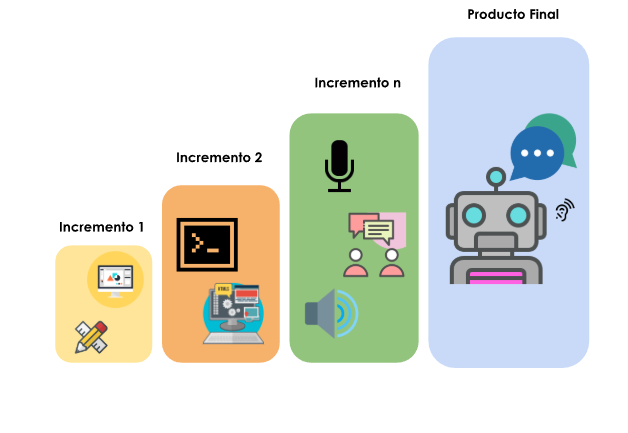
\includegraphics[width=12cm]{figs/incremento}
  \end{center}
  \caption{Método incremental e iterativo}
  \label{fig:incremento}
\end{figure}\


\vspace{0.2cm}

Además, se han realizado reuniones semanales con el tutor del TFG, tanto de forma presencial como mediante Microsoft Teams, para hacer seguimiento de los avances conseguidos y resolver las dudas surgidas durante el desarrollo.




\section{Plan de trabajo}
\label{sec:plantrabajo}

\vspace{0.2cm}

El desarrollo de este proyecto ha constado de diversas etapas, que se describen a continuación:


\begin{enumerate}
	\item \textit{Investigación del estado del arte:} Esta primera etapa se ha centrado en la búsqueda de soluciones existentes al problema planteado. Para ello,  se han consultado plataformas como Google Scholar\footnote{https://scholar.google.es/} y diversos artículos científicos.
	\item \textit{Investigación del hardware a utilizar:} Una vez encontrada una solución factible, se buscaron componentes \textit{hardware} \textit{low-cost}, compatibles con los objetivos planteados.
	\item \textit{Investigación del software a utilizar:} Tras decidir el \textit{hardware} a utilizar, se procedió a seleccionar herramientas \textit{software} compatibles con dicho \textit{hardware} y que no requirieran un elevado coste computacional.
	\item \textit{Diseño del modelo del robot:} Tras definir el diseño del robot, se realizaron prototipos en cartón con el objetivo de comprobar medidas y dimensiones. Una vez validado el diseño, se llevó a cabo el modelado 3D de las piezas mediante la herramienta FreeCAD.
	\item \textit{Impresión de las piezas 3D:} Una vez finalizado el diseño, se procedió a la impresión de las piezas.
	\item \textit{Implementación del software:} El desarrollo del \textit{software} se dividió en subtareas, permitiendo la implementación de las distintas funcionalidades del sistema.
	\item \textit{Prueba del software:} Tras implementar las diferentes parte del \textit{software}, se realizaron pruebas funcionales del sistema completo.
	\item \textit{Prueba del hardware:} Una vez impresas las piezas del robot, se procedió a comprobar el funcionamiento del \textit{hardware} en un entorno real.
	\item \textit{Prueba del sistema final:}  Finalmente, se integraron todos los componentes y se realizaron pruebas del sistema completo, corrigiendo los fallos encontrados.

\end{enumerate}
